\chapter{Linking modern coexistence theory and contemporary niche theory: Appendices S1--S5}
%\chaptermark{Niche and coexistence theory}
%\renewcommand{\sectionmark}[1]{}
\fancyhead[LE, RO]{\thepage}
\fancyhead[RE]{APPENDIX A}
\fancyhead[LO]{NICHE AND COEXISTENCE THEORY}
\fancyfoot{}
\renewcommand{\headrulewidth}{0pt}
\setlength{\parindent}{1cm}


\begin{comment}
\documentclass[hidelinks,12pt]{article}
\usepackage{graphicx,bm, booktabs,lineno,array}
\usepackage[fleqn]{amsmath}
\setlength{\mathindent}{0pt}
\usepackage[compress,comma]{natbib}
\usepackage[a4paper]{geometry}
\usepackage[parfill]{parskip}
\usepackage[usenames,dvipsnames]{color}
\usepackage[font=large,labelfont=bf,margin=1cm, labelsep = none]{caption} % caption formatting
\usepackage{setspace}
\usepackage{gensymb}
\usepackage{color} 
\usepackage{sidecap}
\usepackage{etoolbox}
\newbool{MyRefNumbers}
\usepackage{authblk}
\usepackage{hyperref}
\usepackage[color=cyan]{todonotes}
\pdfminorversion=3
\doublespacing

\newcommand{\plus}{\raisebox{.4\height}{\scalebox{.6}{+}}}
\newcommand{\minus}{\raisebox{.4\height}{\scalebox{.8}{-}}}
\newcommand*\samethanks[1][\value{footnote}]{\footnotemark[#1]}
\newcommand\blfootnote[1]{%
  \begingroup
  \renewcommand\thefootnote{}\footnote{#1}%
  \addtocounter{footnote}{-1}%
  \endgroup
}
\end{comment}



\begin{comment}
\title{Linking modern coexistence theory and contemporary niche theory}
\author[1]{Andrew D. Letten \thanks{These authors contributed equally.}}
\author[1]{Po-Ju Ke \samethanks}
\author[1]{Tadashi Fukami}
\affil[1]{Department of Biology, Stanford University, Stanford, California, 94305-5020, USA}

\begin{document}

\date{}
\maketitle
\singlespacing
\blfootnote{Correspondence email: aletten@stanford.edu, pojuke@stanford.edu, fukamit@stanford.edu}
\textbf{Type of article:} Concepts and Synthesis
\textbf{Running title:} Niche and coexistence theory 
\textbf{Figures:} 6\\
\textbf{Boxes:} 2\\
\newpage
\doublespacing
\linenumbers
\end{comment}



\section{Appendix S1 -- Mathematical derivation of Chesson's niche overlap and fitness differences for consumer--resource models}
To analytically link modern coexistence theory \citep{Chesson2000} and contemporary niche theory \citep{Chase2003}, we translated consumer-resource models into a Lotka--Volterra form following \cite[Ch.~7]{tilman1982}. For a Lotka--Volterra competition model for two consumer species (i.e., $N_{1}$ and $N_{2}$) written as

\begin{equation}
\frac{dN_{1}}{dt}=r_{1}N_{1}\left ( 1-a_{11}N_{1}-a_{12}N_{2} \right ) 
\tag{S2.1.1}\label{eq:S2.1.1}
\end{equation}
\begin{equation}
\frac{dN_{2}}{dt}=r_{2}N_{2}\left ( 1-a_{21}N_{1}-a_{22}N_{2} \right ). 
\tag{S2.1.2}\label{eq:S2.1.2}
\end{equation}

\noindent The model will have an equilibrium density when $N_{1}^{*}=\frac{1}{a_{11}}-\frac{a_{12}}{a_{11}}N_{2}^{*}$ and $N_{2}^{*}=\frac{1}{a_{22}}-\frac{a_{21}}{a_{22}}N_{1}^{*}$. \cite{tilman1982} solved the equilibrium of the consumer-resource model and rearranged it algebraically to a form that is comparable to the equilibrium of a Lotka--Volterra model (an alternative approach to translating consumer-resource models to Lotka--Volterra form involves linearizing inter- and intraspecific density dependences at the equilibrium \citep{Meszenaz2006}, as recently applied in \cite{Kleinhesselink2015}). Note that \cite{tilman1982} parameterized the Lotka--Volterra model in terms of carrying capacities (i.e., $K_{1}$ and $K_{2}$) and relative competition coefficients (i.e., $\alpha$ and $\beta$). His derivation allowed for the rewriting of these parameters in terms of consumer-resource parameters. 
\par


In this appendix, we provide detailed mathematical derivations for two species competing for both perfectly substitutable resources and essential resources. To maintain consistency with modern coexistence theory, we parameterized the Lotka--Volterra model using absolute competition coefficients (i.e., $a_{ij}$). Once the consumer-resource model was translated to a Lotka--Volterra form, we were able to go one step further to quantify Chesson's niche overlap and average fitness difference \citep{Chesson2000, Godoy2014}. 
\par


\subsection*{Mathematical derivation of Chesson's niche overlap and fitness differences for two consumers competing for two substitutable resources}
Following \citet[p.~270]{tilman1982}, the model consists of two resources (i.e., $R_{1}$ and $R_{2}$) that are perfectly nutritionally substitutable for two consumers (i.e., $N_{1}$ and $N_{2}$): 

\begin{equation}
\frac{{d{N_1}}}{{dt}} = {r_1}{N_1}\left[ {\frac{{{w_{11}}{R_1} + {w_{12}}{R_2} - {T_1}}}{{{k_1} + {w_{11}}{R_1} + {w_{12}}{R_2} - {T_1}}}} \right] - D{N_1} 
\tag{S2.2.1}\label{eq:S2.2.1}
\end{equation}
\begin{equation}
\frac{{d{N_2}}}{{dt}} = {r_2}{N_2}\left[ {\frac{{{w_{21}}{R_1} + {w_{22}}{R_2} - {T_2}}}{{{k_2} + {w_{21}}{R_1} + {w_{22}}{R_2} - {T_2}}}} \right] - D{N_2} 
\tag{S2.2.2}\label{eq:S2.2.2}
\end{equation}
\begin{equation}
\frac{{d{R_1}}}{{dt}} = D\left( {{S_1} - {R_1}} \right) - {c_{11}}{N_1} - {c_{21}}{N_2} \tag{S2.2.3}\label{eq:S2.2.3}
\end{equation}
\begin{equation}
\frac{{d{R_2}}}{{dt}} = D\left( {{S_2} - {R_2}} \right) - {c_{12}}{N_1} - {c_{22}}{N_2}.
\tag{S2.2.4}\label{eq:S2.2.4}
\end{equation}

\noindent Here, $r_{i}$ represents the maximum population growth rate for species $i$ ($i = $ 1 or 2) and $D$ represents the constant mortality of the consumers and turnover rate of resources. Per capita resource consumption rate of consumer $N_{i}$ on resource $R_{j}$ ($j = $ 1 or 2) is represented by $c_{ij}$, whereas $w_{ij}$ represents a weighting factor that converts availability of $R_{j}$ into its value for consumer $N_{i}$. Following a Monod growth model, $k_{i}$ is the half-saturation constant for $N_{i}$ resource consumption, and $T_{i}$ is the minimum amount of total resource required for $N_{i}$ to grow. Finally, $S_{1}$ and $S_{2}$ represent the resource supply concentrations for $R_{1}$ and $R_{2}$, respectively. As noted in \cite{Kleinhesselink2015}, certain assumptions of this Monod growth model, such as constant supply of resource and strong recipient control of consumption rate, may not be applicable to many systems. However, this should not affect the results qualitatively.
\par


By setting Eqns.~\ref{eq:S2.2.1} and \ref{eq:S2.2.2} to zero, we solved the zero net growth isolines (ZNGI) of consumers, which represent resource combinations of $R_{1}$ and $R_{2}$ that cause consumers' growth equal to its mortality, as:

\begin{equation}
R_2 =  - \frac{{{w_{11}}}}{{{w_{12}}}}R_1 + {B_1} 
\tag{S2.3.1}\label{eq:S2.3.1}
\end{equation}
\begin{equation}
R_2 =  - \frac{{{w_{21}}}}{{{w_{22}}}}R_1 + {B_2}, 
\tag{S2.3.2}\label{eq:S2.3.2}
\end{equation}

\noindent where ${B_1} = \left[ {\frac{{D\left( {{k_1} - {T_1}} \right) + {r_1}{T_1}}}{{{w_{12}}\left( {{r_1} - D} \right)}}} \right]$, and ${B_2} = \left[ {\frac{{D\left( {{k_2} - {T_2}} \right) + {r_2}{T_2}}}{{{w_{21}}\left( {{r_2} - D} \right)}}} \right]\left( {\frac{{{w_{21}}}}{{{w_{22}}}}} \right)$. Given that the ZNGI of $N_{1}$ and $N_{2}$ must cross to ensure coexistence of consumers, the equilibrium resource densities, $R_{1}^{*}$ and $R_{2}^{*}$, were solved as:

\begin{equation}
R_1^* = {{\left( {{B_1} - {B_2}} \right)} \mathord{\left/
		{\vphantom {{\left( {{B_1} - {B_2}} \right)} {\left( {\frac{{{w_{11}}}}{{{w_{12}}}} - \frac{{{w_{21}}}}{{{w_{22}}}}} \right)}}} \right.
		\kern-\nulldelimiterspace} {\left( {\frac{{{w_{11}}}}{{{w_{12}}}} - \frac{{{w_{21}}}}{{{w_{22}}}}} \right)}} 
\tag{S2.4.1}\label{eq:S2.4.1}
\end{equation}
\begin{equation}
R_2^* = {{\left( {{B_1}\frac{{{w_{12}}}}{{{w_{11}}}} - {B_2}\frac{{{w_{22}}}}{{{w_{21}}}}} \right)} \mathord{\left/
		{\vphantom {{\left( {{B_1}\frac{{{w_{12}}}}{{{w_{11}}}} - {B_2}\frac{{{w_{22}}}}{{{w_{21}}}}} \right)} {\left( {\frac{{{w_{21}}}}{{{w_{11}}}} - \frac{{{w_{22}}}}{{{w_{21}}}}} \right)}}} \right.
		\kern-\nulldelimiterspace} {\left( {\frac{{{w_{12}}}}{{{w_{11}}}} - \frac{{{w_{22}}}}{{{w_{21}}}}} \right)}}.
\tag{S2.4.2}\label{eq:S2.4.2}
\end{equation}

\noindent By substituting the equilibrium resource densities into Eqns.~\ref{eq:S2.2.3} and \ref{eq:S2.2.4}, we obtained the equilibrium consumer densities, $N_{1}^{*}$ and $N_{2}^{*}$. The consumer equilibrium density can be written in a form comparable to that of the Lotka--Volterra model. For $N_{1}$, the specific form of its equilibrium density can be derived by Eqn.~\ref{eq:S2.2.3} $\times \frac{w_{11}}{w_{12}} + $ Eqn.~\ref{eq:S2.2.4}:

\begin{equation}
N_1^* = \left[ {\frac{{D\left( {{S_2} + \frac{{{w_{11}}}}{{{w_{12}}}}{S_1} - {B_1}} \right)}}{{{c_{12}} + {c_{11}}\frac{{{w_{11}}}}{{{w_{12}}}}}}} \right] - \left[ {\frac{{{c_{22}} + {c_{21}}\frac{{{w_{11}}}}{{{w_{12}}}}}}{{{c_{12}} + {c_{11}}\frac{{{w_{11}}}}{{{w_{12}}}}}}} \right]N_2^*. 
\tag{S2.5}\label{eq:S2.5}
\end{equation}

Eqn.~\ref{eq:S2.5} consists of a first component with only $N_{1}$-related parameters, and a heterospecific density-dependent component which decreases with its competitor's density (i.e., $N_{2}^{*}$). Note that the specific algebraic treatment applied to obtain Eqn.~\ref{eq:S2.5} served the purpose to generate the density-independent component independent of parameters of the competitor. By comparing this expression with $N_{1}^{*}=\frac{1}{a_{11}}-\frac{a_{12}}{a_{11}}N_{2}^{*}$, the algebraic equivalents for $a_{11}$ and $a_{12}$ are:

\begin{equation}
{a_{11}} = \frac{{{c_{12}} + {c_{11}}\frac{{{w_{11}}}}{{{w_{12}}}}}}{{D\left( {{S_2} + \frac{{{w_{11}}}}{{{w_{12}}}}{S_1} - {B_1}} \right)}}
\tag{S2.6.1}\label{eq:S2.6.1}
\end{equation}
\begin{equation}
{a_{12}} = \frac{{{c_{22}} + {c_{21}}\frac{{{w_{11}}}}{{{w_{12}}}}}}{{D\left( {{S_2} + \frac{{{w_{11}}}}{{{w_{12}}}}{S_1} - {B_1}} \right)}}.
\tag{S2.6.2}\label{eq:S2.6.2}
\end{equation}

\noindent For $N_{2}$, its equilibrium density can be derived by Eqn.~\ref{eq:S2.2.3}$\times \frac{w_{21}}{w_{22}} + $ Eqn.~\ref{eq:S2.2.4}:

\begin{equation}
N_2^* = \left[ {\frac{{D\left( {{S_2} + \frac{{{w_{21}}}}{{{w_{22}}}}{S_1} - {B_2}} \right)}}{{{c_{22}} + {c_{21}}\frac{{{w_{21}}}}{{{w_{22}}}}}}} \right] - \left[ {\frac{{{c_{12}} + {c_{11}}\frac{{{w_{21}}}}{{{w_{22}}}}}}{{{c_{22}} + {c_{21}}\frac{{{w_{21}}}}{{{w_{22}}}}}}} \right]N_1^*.
\tag{S2.7}\label{eq:S2.7}
\end{equation}

Similar to Eqn.~\ref{eq:S2.5}, Eqn.~\ref{eq:S2.7} consists of a density-independent component with only $N_{2}$-related parameters, and a heterospecific density-dependent component which decreases with the density of $N_{1}^{*}$. By comparing Eqn.~\ref{eq:S2.7} with $N_{2}^{*}=\frac{1}{a_{22}}-\frac{a_{21}}{a_{22}}N_{1}^{*}$, the algebraic equivalents for $a_{22}$ and $a_{21}$ are:

\begin{equation}
{a_{22}} = \frac{{{c_{22}} + {c_{21}}\frac{{{w_{21}}}}{{{w_{22}}}}}}{{D\left( {{S_2} + \frac{{{w_{21}}}}{{{w_{22}}}}{S_1} - {B_2}} \right)}} 
\tag{S2.8.1}\label{eq:S2.8.1}
\end{equation}
\begin{equation}
{a_{21}} = \frac{{{c_{12}} + {c_{11}}\frac{{{w_{21}}}}{{{w_{22}}}}}}{{D\left( {{S_2} + \frac{{{w_{21}}}}{{{w_{22}}}}{S_1} - {B_2}} \right)}}.
\tag{S2.8.2}\label{eq:S2.8.2}
\end{equation}

Chesson defines niche overlap as $\rho=\sqrt {\frac{{{a_{12}}{a_{21}}}}{{{a_{11}}{a_{22}}}}}$ and absolute fitness difference of $N_{2}$ over $N_{1}$ as $\frac{{{f_2}}}{{{f_1}}} = \sqrt {\frac{{{a_{11}}{a_{12}}}}{{{a_{22}}{a_{21}}}}}$ \citep{Chesson2013ecosys}. By writing out the absolute competition coefficients in terms of consumer-resource parameters (i.e., Eqns.~\ref{eq:S2.6.1} -- \ref{eq:S2.6.2} and Eqns.~\ref{eq:S2.8.1} -- \ref{eq:S2.8.2}), we can express the niche overlap as: 

\begin{equation}
\rho  = \sqrt {\frac{{{a_{12}}{a_{21}}}}{{{a_{11}}{a_{22}}}}}  = \sqrt {\frac{\left (
		c_{22} + c_{21}\frac{w_{11}}{w_{12}}\right )\left ( 
		c_{12} + c_{11}\frac{w_{21}}{w_{22}} \right )}{\left (
		c_{12} + c_{11}\frac{w_{11}}{w_{12}}\right )\left ( 
		c_{22} + c_{21}\frac{w_{21}}{w_{22}} \right )}} 
\tag{S2.9}\label{eq:S2.9}
\end{equation}
and the absolute fitness difference of $N_{2}$ over $N_{1}$ as:
\begin{equation}
\frac{{{f_2}}}{{{f_1}}} = \sqrt {\frac{{{a_{11}}{a_{12}}}}{{{a_{22}}{a_{21}}}}}  = \frac{\left (S_{2}+\frac{w_{21}}{w_{22}}S_{1}-B_{2}\right )}{\left (S_{2}+\frac{w_{11}}{w_{12}}S_{1}-B_{1}\right )}\sqrt {\frac{\left (
		c_{12} + c_{11}\frac{w_{11}}{w_{12}}\right )\left ( 
		c_{22} + c_{21}\frac{w_{11}}{w_{12}} \right )}{\left (
		c_{22} + c_{21}\frac{w_{21}}{w_{22}}\right )\left ( 
		c_{12} + c_{11}\frac{w_{21}}{w_{22}} \right )}}.
\tag{S2.10}\label{eq:2.10}
\end{equation}


\subsection*{Mathematical derivation of Chesson's niche overlap and fitness differences for two consumers competing for two essential resources} 
We applied the same mathematical techniques for a consumer-resource model where the resources are essential, which takes the general form as follows \citep{tilman1982}: 

\begin{equation}
\frac{{d{N_1}}}{{dt}} = {r_1}{N_1}\min \left[ {\frac{{{R_1}}}{{{R_1} + {k_{11}}}},{\rm{ }}\frac{{{R_2}}}{{{R_2} + {k_{12}}}}} \right] - {m_1}{N_1} 
\tag{S2.11.1}\label{eq:S2.11.1}
\end{equation}
\begin{equation}
\frac{{d{N_2}}}{{dt}} = {r_2}{N_2}\min \left[ {\frac{{{R_1}}}{{{R_1} + {k_{21}}}},{\rm{ }}\frac{{{R_2}}}{{{R_2} + {k_{22}}}}} \right] - {m_2}{N_2}
\tag{S2.11.2}\label{eq:S2.11.2}
\end{equation}
\begin{equation}
\frac{{d{R_1}}}{{dt}} = D\left( {{S_1} - {R_1}} \right) - {c_{11}}\left( {\frac{{d{N_1}}}{{dt}} + {m_1}{N_1}} \right) - {c_{21}}\left( {\frac{{d{N_2}}}{{dt}} + {m_2}{N_2}} \right)
\tag{S2.11.3}\label{eq:S2.11.3}
\end{equation}
\begin{equation}
\frac{{d{R_2}}}{{dt}} = D\left( {{S_2} - {R_2}} \right) - {c_{12}}\left( {\frac{{d{N_1}}}{{dt}} + {m_1}{N_1}} \right) - {c_{22}}\left( {\frac{{d{N_2}}}{{dt}} + {m_2}{N_2}} \right).
\tag{S2.11.4}\label{eq:S2.11.4}
\end{equation}

\noindent Here, $m_1$ and $m_2$ represent mortality rates for consumers $N_1$ and $N_2$, respectively, whereas other parameter notations are the same as Eqns.~\ref{eq:S2.2.1} -- \ref{eq:S2.2.4}. In order to keep consistency with \cite[Ch.~7]{tilman1982}, we applied the following specific model for our analysis:  

\begin{equation}
\frac{{d{N_1}}}{{dt}} = {r_1}{N_1}\min \left[ {\frac{{{R_1}}}{{{R_1} + {k_{11}}}},{\rm{ }}\frac{{{R_2}}}{{{R_2} + {k_{12}}}}} \right] - {m_1}{N_1}
\tag{S2.12.1}\label{eq:S2.12.1}
\end{equation}
\begin{equation}
\frac{{d{N_2}}}{{dt}} = {r_2}{N_2}\min \left[ {\frac{{{R_1}}}{{{R_1} + {k_{21}}}},{\rm{ }}\frac{{{R_2}}}{{{R_2} + {k_{22}}}}} \right] - {m_2}{N_2}
\tag{S2.12.2}\label{eq:S2.12.2}
\end{equation}
\begin{equation}
\frac{{d{R_1}}}{{dt}} = D\left( {{S_1} - {R_1}} \right) - {c_{11}}{N_{1}} - {c_{21}}{N_{2}}
\tag{S2.12.3}\label{eq:S2.12.3}
\end{equation}
\begin{equation}
\frac{{d{R_2}}}{{dt}} = D\left( {{S_2} - {R_2}} \right) - {c_{12}}{N_{1}} - {c_{22}}{N_{2}}.
\tag{S2.12.4}\label{eq:S2.12.4}
\end{equation}

\noindent As mentioned in the main text, nutrient limitation status due to resource availability depends on the relative position of the resource supply point, the monocultural resource equilibrium (i.e., $R_{ij}^{*}$), and the consumption vector. When translating the essential consumer-resource model to Lotka--Volterra form, we thus need to consider the nutrient limitation status of each species (Fig.~\ref{fig:supply-ms-fig}c). By drawing a line from each species' $R_{ij}^{*}$ parallel to its consumption vector, we can partition the resource supply space into three sections: (i) both $N_{1}$ and $N_{2}$ are limited by $R_{1}$ (i.e., beyond the blue dotted lines), (ii) $N_{1}$ is limited by $R_{2}$ and $N_{2}$ is limited by $R_{1}$ (i.e., between the blue and red dotted line), and (iii) both $N_{1}$ and $N_{2}$ are limited by $R_{2}$ (i.e., below the red dotted lines) (Fig.~\ref{fig:supply-ms-fig}c). Here, we demonstrate how Chesson's niche overlap and fitness difference can be quantified in an essential resource model by focusing on region (ii), where the two species are limited by different resources at the equilibrium. In this region, Eqns.~\ref{eq:S2.12.1} -- \ref{eq:S2.12.4} becomes:

\begin{equation}
\frac{{d{N_1}}}{{dt}} = {r_1}{N_1} \left[{\frac{{{R_2}}}{{{R_2} + {k_{12}}}}} \right] - {m_1}{N_1}
\tag{S2.13.1}\label{eq:S2.13.1}
\end{equation}
\begin{equation}
\frac{{d{N_2}}}{{dt}} = {r_2}{N_2} \left[{\frac{{{R_1}}}{{{R_1} + {k_{21}}}}} \right] - {m_2}{N_2}
\tag{S2.13.2}\label{eq:S2.13.2}
\end{equation}
\begin{equation}
\frac{{d{R_1}}}{{dt}} = D\left( {{S_1} - {R_1}} \right) - {c_{11}}{N_{1}} - {c_{21}}{N_{2}}
\tag{S2.13.3}\label{eq:S2.13.3}
\end{equation}
\begin{equation}
\frac{{d{R_2}}}{{dt}} = D\left( {{S_2} - {R_2}} \right) - {c_{12}}{N_{1}} - {c_{22}}{N_{2}}.
\tag{S2.13.4}\label{eq:S2.13.4}
\end{equation}

As in the substitutable resource model, we solved for the equilibrium resource densities. While this is represented as the ZNGI in the substitutable resource model, here we can directly solve for $R_{2}^{*}$ (defined as $R_{12}^{*}$) from Eqn.~\ref{eq:S2.13.1} and $R_{1}^{*}$ (defined as $R_{21}^{*}$) from Eqn.~\ref{eq:S2.13.2} as:

\begin{equation}
R_{12}^{*}=\frac{m_{1}k_{12}}{r_{1}-m_{1}}
\tag{S2.14.1}\label{eq:S2.14.1}
\end{equation}
\begin{equation}
R_{21}^{*}=\frac{m_{2}k_{21}}{r_{2}-m_{2}}.
\tag{S2.14.2}\label{eq:S2.14.2}
\end{equation}

Substituting Eqns.~\ref{eq:S2.14.1} and \ref{eq:S2.14.2} back to Eqns.~\ref{eq:S2.13.3} and \ref{eq:S2.13.4} respectively allows us to solve the equilibrium for $N_{1}$ and $N_{2}$ as:

\begin{equation}
N_{1}^{*}=\frac{D}{c_{12}}\left ( S_{2}-{R_{12}^{*}} \right )-\frac{c_{22}}{c_{12}}N_{2}^{*}
\tag{S2.15.1}\label{eq:S2.15.1}
\end{equation}
\begin{equation}
N_{2}^{*}=\frac{D}{c_{21}}\left ( S_{1}-{R_{21}^{*}} \right )-\frac{c_{11}}{c_{21}}N_{1}^{*}.
\tag{S2.15.2}\label{eq:S2.15.2}
\end{equation}

\noindent By comparing Eqns.\ref{eq:S2.15.1} and \ref{eq:S2.15.2} to $N_{1}^{*}=\frac{1}{a_{11}}-\frac{a_{12}}{a_{11}}N_{2}^{*}$ and $N_{2}^{*}=\frac{1}{a_{22}}-\frac{a_{21}}{a_{22}}N_{1}^{*}$, respectively, we find $a_{11}$, $a_{12}$, $a_{21}$, and $a_{22}$ for the essential resource model in region (ii):

\begin{equation}
a_{11}=\frac{c_{12}}{D\left ( S_{2}-R_{12}^{*} \right )}
\tag{S2.16.1}\label{eq:S2.16.1}
\end{equation}
\begin{equation}
a_{12}=\frac{c_{22}}{D\left ( S_{2}-R_{12}^{*} \right )}
\tag{S2.16.2}\label{eq:S2.16.2}
\end{equation}
\begin{equation}
a_{21}=\frac{c_{11}}{D\left ( S_{1}-R_{21}^{*} \right )}
\tag{S2.16.3}\label{eq:S2.16.3}
\end{equation}
\begin{equation}
a_{22}=\frac{c_{21}}{D\left ( S_{1}-R_{21}^{*} \right )}.
\tag{S2.16.4}\label{eq:S2.16.4}
\end{equation}

\noindent Following similar methods, we solved for each of Chesson's components in regions where both species are limited by the same resource. For region (i), where both species are $R_{1}$-limited, 

\begin{equation}
a_{11}=\frac{c_{11}}{D\left ( S_{1}-R_{11}^{*} \right )}
\tag{S2.17.1}\label{eq:S2.17.1}
\end{equation} 
\begin{equation}
a_{12}=\frac{c_{21}}{D\left ( S_{1}-R_{11}^{*} \right )}
\tag{S2.17.2}\label{eq:S2.17.2} 
\end{equation}
\begin{equation}
a_{21}=\frac{c_{11}}{D\left ( S_{1}-R_{21}^{*} \right )}
\tag{S2.17.3}\label{eq:S2.17.3}
\end{equation}
\begin{equation}
a_{22}=\frac{c_{21}}{D\left ( S_{1}-R_{21}^{*} \right )}.
\tag{S2.17.4}\label{eq:S2.17.4}
\end{equation}

\noindent For region (iii), where both species are $R_{2}$-limited, 

\begin{equation}
a_{11}=\frac{c_{12}}{D\left ( S_{2}-R_{12}^{*} \right )}
\tag{S2.18.1}\label{eq:S2.18.1}
\end{equation}
\begin{equation}
a_{12}=\frac{c_{22}}{D\left ( S_{2}-R_{12}^{*} \right )}
\tag{S2.18.2}\label{eq:S2.18.2}
\end{equation}
\begin{equation}
a_{21}=\frac{c_{12}}{D\left ( S_{2}-R_{22}^{*} \right )}
\tag{S2.18.3}\label{eq:S2.18.3}
\end{equation}
\begin{equation}
a_{22}=\frac{c_{22}}{D\left ( S_{2}-R_{22}^{*} \right )}.
\tag{S2.18.4}\label{eq:S2.18.4}
\end{equation}



\section{Appendix S2 -- Analytical form and positivity criteria of $E_{Ni}^{*}$}
In this study we used Tilman's consumer-resource model for substitutable resources (i.e., Appendix A, Eqns.~\ref{eq:S2.2.1} -- \ref{eq:S2.2.4}) following \cite[p.~270]{tilman1982}, which has also been applied in many other studies (e.g., \cite{Meszenaz2006}, \cite{Barabas2014}). As pointed out by \cite{Kleinhesselink2015}, this model assumes that resource uptake is proportional only to consumer abundance. The structure of this model may result in negative resource equilibrium values, especially under the scenario where one species excludes the other (i.e., the mono-dominance equilibrium). As mentioned in the main text, our simulations were performed in parameter regions that only resulted in positive resource equilibrium values. Here, we further supplement this argument with analytical solutions for this particular model. We first derived the analytical solution of the equilibrium when $N_1$ outcompetes $N_2$ (hereafter termed \textbf{$E_{N1}^{*}$}), and when $N_2$ outcompetes $N_1$ (hereafter termed \textbf{$E_{N2}^{*}$}). We then derived the criteria for positive resource equilibrium and listed the parameters used for the simulations. 
\par


\subsection*{Analytical form and positivity criteria of $E_{N1}^{*}$} 
Under \textbf{$E_{N1}^{*}$} ($N_{1}^{*} >$  0, $N_{2}^{*}$ = 0), by setting Eqns.~\ref{eq:S2.2.3} and \ref{eq:S2.2.4} equal to zero, we derived Eqns.~\ref{eq:S2.19.1} and \ref{eq:S2.19.2}, respectively:

\begin{equation}
R_{1}^{*} = S_1-\frac{c_{11}}{D}N_{1}^{*}
\tag{S2.19.1}\label{eq:S2.19.1}
\end{equation}
\begin{equation}
R_{2}^{*} = S_2-\frac{c_{12}}{D}N_{1}^{*}.
\tag{S2.19.2}\label{eq:S2.19.2}
\end{equation}

\noindent By substituting Eqns.~\ref{eq:S2.19.1} and \ref{eq:S2.19.2} into Eqns.~\ref{eq:S2.2.1}, $N_{1}^{*}$ can be derived as follows:

\begin{equation}
N_{1}^{*} = D\left [\frac{\left ( r_1 - D\right )\left ( w_{11}S_{1}+w_{12}S_{2}-T_{1} \right )-Dk_{1}}{\left ( r_1-D \right )\left (  w_{11}c_{11}+w_{12}c_{12} \right )}\right].
\tag{S2.20}\label{eq:S2.20}
\end{equation}

\noindent For $R_{1}^{*}$ and $R_{2}^{*}$ to be positive, the following two inequalities should be fulfilled respectively:

\begin{equation}
S_1\left ( r_{1}-D \right )w_{12}c_{12} - S_2\left ( r_1-D \right )w_{12}c_{11} > -\left ( r_{1}-D \right )c_{11}T_{1} - Dk_{1}c_{11}
\tag{S2.21.1}\label{eq:S2.21.1}
\end{equation}
\begin{equation}
S_1\left ( r_{1}-D \right )w_{11}c_{12} - S_2\left ( r_1-D \right )w_{11}c_{11} < \left ( r_{1}-D \right )c_{12}T_{1} - Dk_{1}c_{12}.
\tag{S2.21.2}\label{eq:S2.21.2}
\end{equation}

By combining criteria \ref{eq:S2.21.1} and \ref{eq:S2.21.2}, we derived the criteria for positive resource equilibrium under $E_{N1}^{*}$:

\begin{equation}
\frac{-1}{w_{12}c_{12}}\left [ T_{1} + \frac{Dk_{1}}{\left ( r_{1}-D \right )}\right ] < \frac{S_1}{c_{11}}-\frac{S_2}{c_{12}} < \frac{1}{w_{11}c_{11}}\left [ T_{1} + \frac{Dk_{1}}{\left ( r_{1}-D \right )}\right ].
\tag{S2.22}\label{eq:S2.22}
\end{equation}



\subsection*{Analytical form and positivity criteria of $E_{N2}^{*}$} 
Following similar mathematical logic, we derived the analytical form of $E_{N2}^{*}$ ($N_{1}^{*} =$  0, $N_{2}^{*} >$ 0) as follows:

\begin{equation}
N_{2}^{*} = D\left [\frac{\left ( r_2 - D\right )\left ( w_{21}S_{1}+w_{22}S_{2}-T_{2} \right )-Dk_{2}}{\left ( r_2-D \right )\left (  w_{21}c_{21}+w_{22}c_{22} \right )}\right],
\tag{S2.23.1}\label{eq:S2.23.1}
\end{equation}
\begin{equation}
R_{1}^{*} = S_1-\frac{c_{21}}{D}N_{2}^{*}
\tag{S2.23.2}\label{eq:S2.23.2}
\end{equation}
\begin{equation}
R_{2}^{*} = S_2-\frac{c_{22}}{D}N_{2}^{*}.
\tag{S2.23.3}\label{eq:S2.23.3}
\end{equation}

\noindent We then obtained the positivity criteria for $R_{1}^{*}$ and $R_{2}^{*}$ under $E_{N2}^{*}$. That is, both $S_1/c_{21}$ and $S_2/c_{22}$ need to be greater than the term within the bracket of Eqn.\ref{eq:S2.23.1}. By combining the resulting inequalities, we derived the criteria for positive resource equilibrium as:

\begin{equation}
\frac{-1}{w_{22}c_{22}}\left [ T_{2} + \frac{Dk_{2}}{\left ( r_{2}-D \right )}\right ] < \frac{S_1}{c_{21}}-\frac{S_2}{c_{22}} < \frac{1}{w_{21}c_{21}}\left [ T_{2} + \frac{Dk_{2}}{\left ( r_{2}-D \right )}\right ].
\tag{S2.24}\label{eq:S2.24}
\end{equation}

Based on the positivity criteria (i.e., inequality \ref{eq:S2.22} and \ref{eq:S2.24}), we used the following values for our analysis of the substitutable resource model: $D=0.5$, $c_{11}=2$, $c_{12}=4$, $c_{21}=4$, $c_{2}=2$, $w_{11}=2$, $w_{12}=4$, $w_{21}=4$, $w_{2}=2$, $k_{1}=k_{2}=0.4$, $r_{1}=r_{2}=1$, $T_{1}=T_{2}=0.05$. For Fig.~\ref{fig:supply-ms-fig} (i.e., changing resource supply ratio) in the main text, $S_1$ and $S_2$ were varied between 0.168 and 0.432. For Fig.~\ref{fig:impact-ms-fig} (i.e., changing impact niche overlap) and Fig.~\ref{fig:require-ms-fig-fixedequilibrium} (i.e., changing requirement niche overlap), $\left ( S_{1}, S_{2} \right )$ were set as (0.28, 0.22) and (0.2, 0.15), respectively. For the essential resource model, $w_{11}=2$; $w_{12}=4$; $w_{21}=4$; $w_{2}=2$ were used. Resource supply rates $\left ( S_{1}, S_{2} \right )$ were varied between 0.25 and 0.75 for Fig.~\ref{fig:supply-ms-fig}, and set as (0.75, 0.55) and (0.4, 0.32) for Figs.~\ref{fig:impact-ms-fig} and \ref{fig:require-ms-fig-fixedequilibrium}, respectively. 



\clearpage
\section{Appendix S3 -- The effect of changing impact niche overlap asymmetrically}
Here, we show the effect on Chesson's niche overlap and fitness difference when impact niche overlap is changed asymmetrically, by holding one species' impact vector constant while modifying the impact vector of its competitor. 
\par


\begin{figure}[H]
	\centering
	\makebox[\textwidth][c]{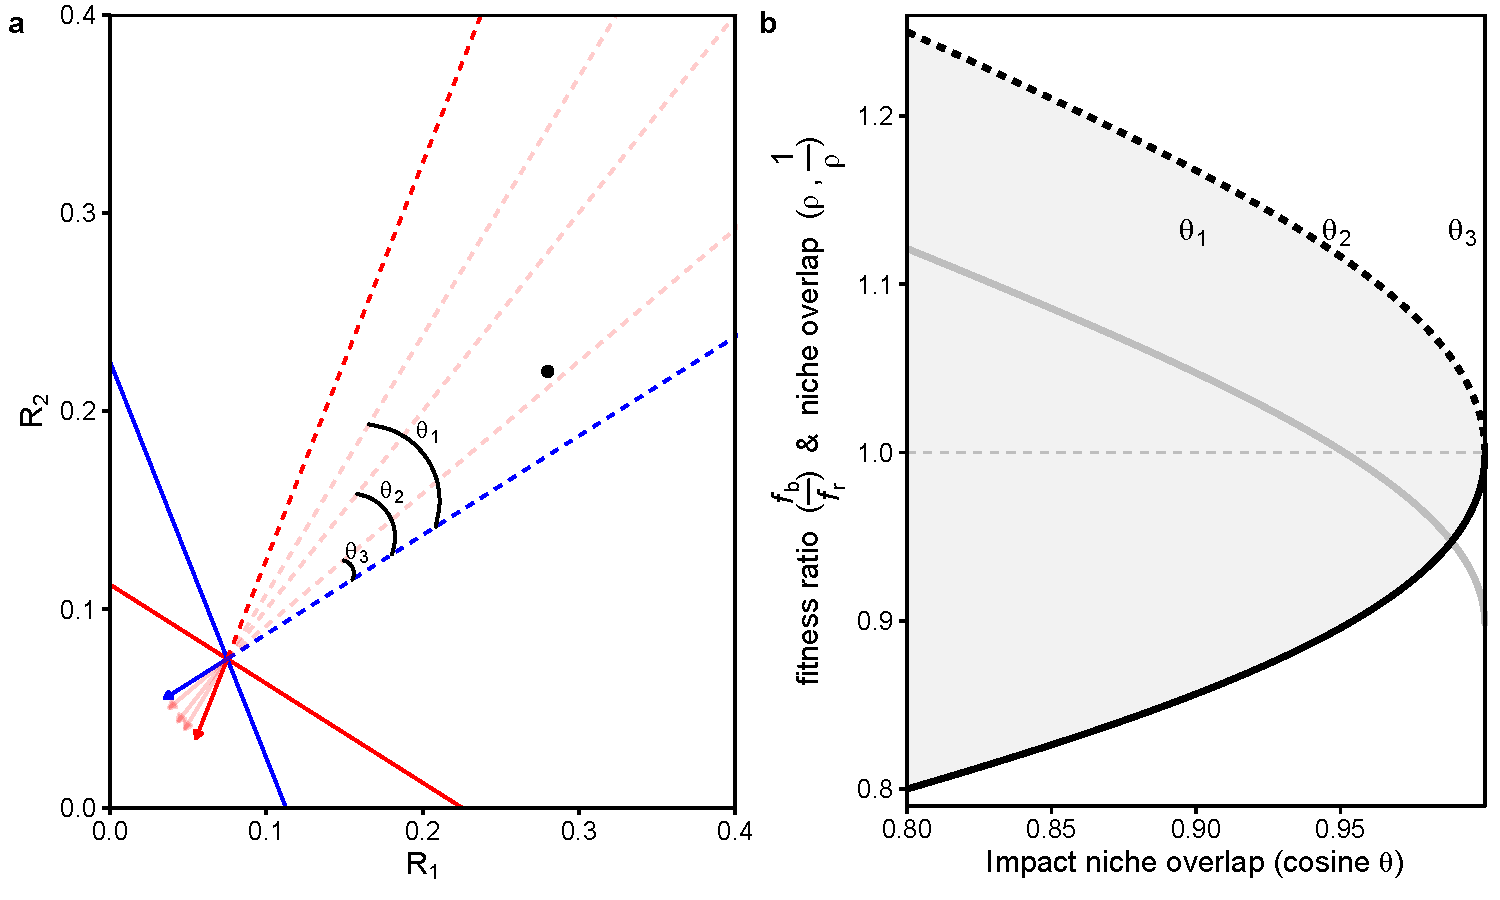
\includegraphics[width=12cm]{Chapter2/impact-appendix-fig-asymmetry-update.pdf}}
	\caption[The effect of changing impact niche overlap asymmetrically under pairwise competition for substitutable resources.]
		{\hspace{1mm}The effect of changing impact niche overlap asymmetrically under pairwise competition for substitutable resources. In (a), the solid red and blue lines are the ZNGIs for each species; the solid lines with arrow heads are the respective impact vectors; and the dashed lines are the inverse of the impact vectors, defining regions of stable coexistence. In (b), the x-axis represents the impact niche overlap starting from the position given by the solid bold impact vectors in (a) and ending at complete overlap. The y-axis gives the values of the fitness differences term, $f_{b}/f_{r}$ (solid grey line), and the degree of niche overlap, $\rho$ (solid black line) and $1/\rho$ (dashed black line). The grey shaded area indicates the coexistence region, where $\rho<f_{b}/f_{r}<1/\rho$. For reference, equal fitness, where $f_{b}/f_{r}=1$, is illustrated by the horizontal dashed grey line. The angles given by $\theta_{1-3}$ in (a) correspond to the respective $\theta_{1-3}$ in (b).}
	\label{fig:impact-appendix-fig-asymmetry}
\end{figure}



\clearpage
\section{Appendix S4 -- The effect of rotating the impact vectors whilst holding impact niche overlap constant}
Here, we show the effect on Chesson's niche overlap and fitness differences of rotating the impact vectors in a common direction whilst holding impact niche overlap constant. Note that the non-monotonic change in Chesson's niche overlap is an artifact of non-linearities in converting angular change into vectors. Because we used trigonometric functions (sine and cosine) to obtain new coordinates for the impact vectors while rotating them, the conversion from angles to coordinates was necessarily non-linear. More specifically, the rate of increase in the sine function decreases in the direction from 0 to 90 degrees, while the rate of decrease in the cosine function increases in the direction from 0 to 90 degrees. The implication of this is that although the angle defining impact niche overlap is held constant, there is a slight decoupling in the rates of change of the vector coordinates that are used in the mechanistic definition of Chesson's niche overlap term. This decoupling means that the rate at which the two species change in their impacts is not identical, which in turn translates into a spurious change in Chesson's niche overlap.  
\par


\newpage
\begin{figure}[H]
	\centering
	\makebox[\textwidth][c]{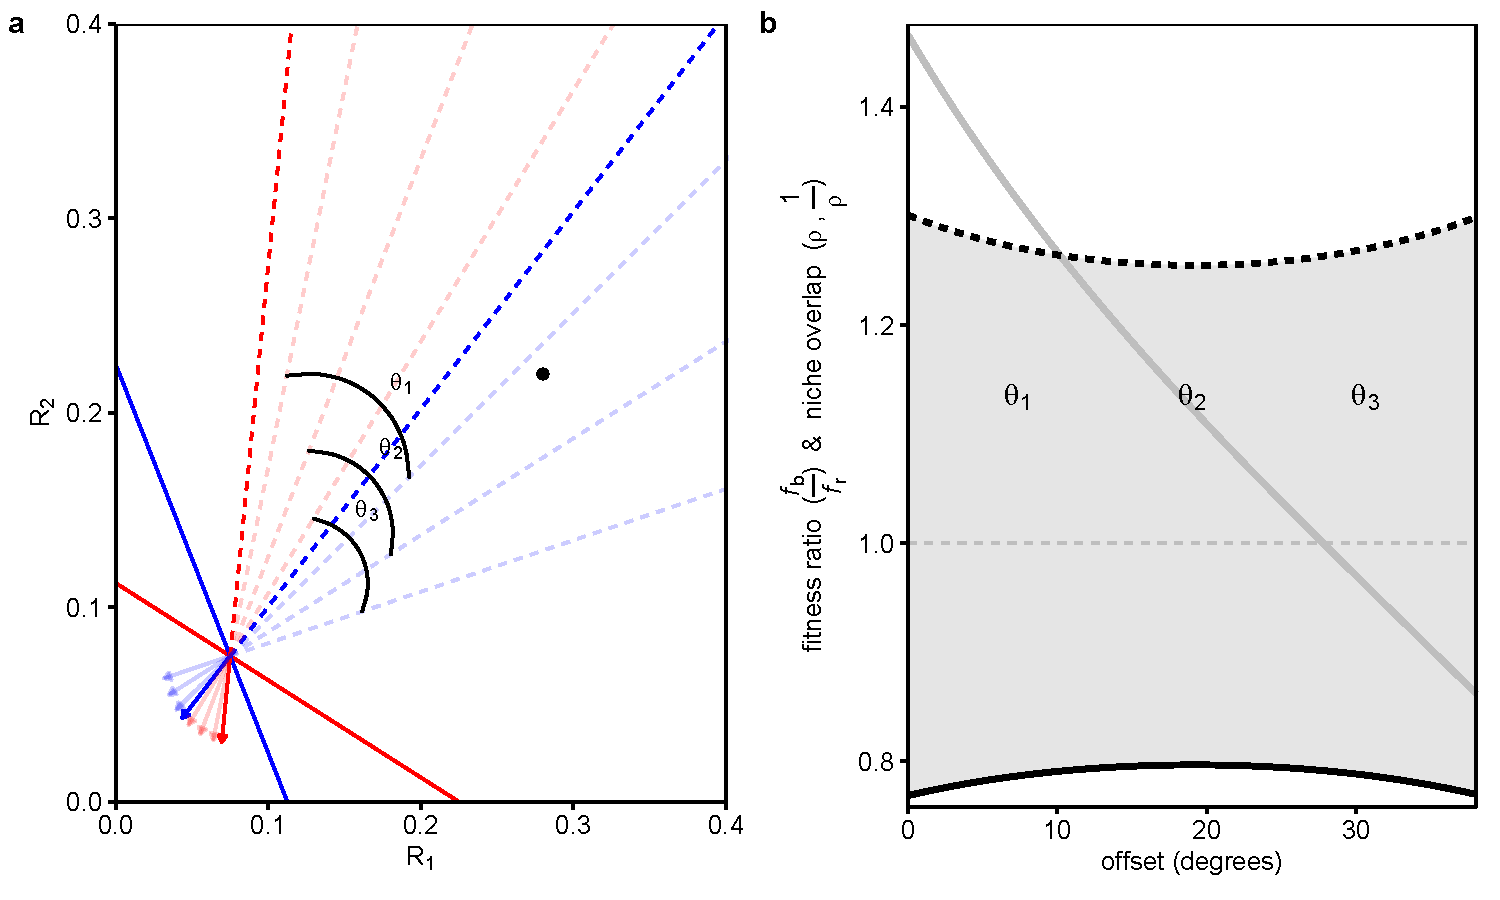
\includegraphics[width=12cm]{Chapter2/impact-ms-fig-fixed-overlap-appendix.pdf}}
	\caption[The effect of rotating the impact vectors in a common direction whilst holding impact niche overlap constant, under pairwise competition for substitutable resources.]
		{\hspace{1mm}The effect of rotating the impact vectors in a common direction whilst holding impact niche overlap constant, under pairwise competition for substitutable resources. In (a), the solid red and blue lines are the ZNGIs for each species; the solid lines with arrow heads are the respective impact vectors; and the dashed lines are the inverse of the impact vectors, defining regions of stable coexistence. In (b), the x-axis represents degrees that the impact vectors are rotated through starting from the position given by the solid bold impact vectors in (a). The y-axis gives the values of the fitness differences term, $f_{b}/f_{r}$ (solid grey line), and the degree of niche overlap, $\rho$ (solid black line) and $1/\rho$ (dashed black line). The grey shaded area indicates the coexistence region, where $\rho<f_{b}/f_{r}<1/\rho$. For reference, equal fitness, where $f_{b}/f_{r}=1$, is illustrated by the horizontal dashed grey line. The angles given by $\theta_{1-3}$ in (a) correspond to the respective $\theta_{1-3}$ in (b).}
	\label{fig:impact-appendix-fig-fix}
\end{figure}



\clearpage
\section{Appendix S5 -- The effects of changing requirement niche overlap without fixing the equilibrium resource density for the essential resources model}
Here, we show the effect on Chesson's niche overlap and fitness difference of changing ZNGIs without fixing the resource equilibrium under competition for essential resources.
\par


\begin{figure}[H]
	\centering
	\makebox[\textwidth][c]{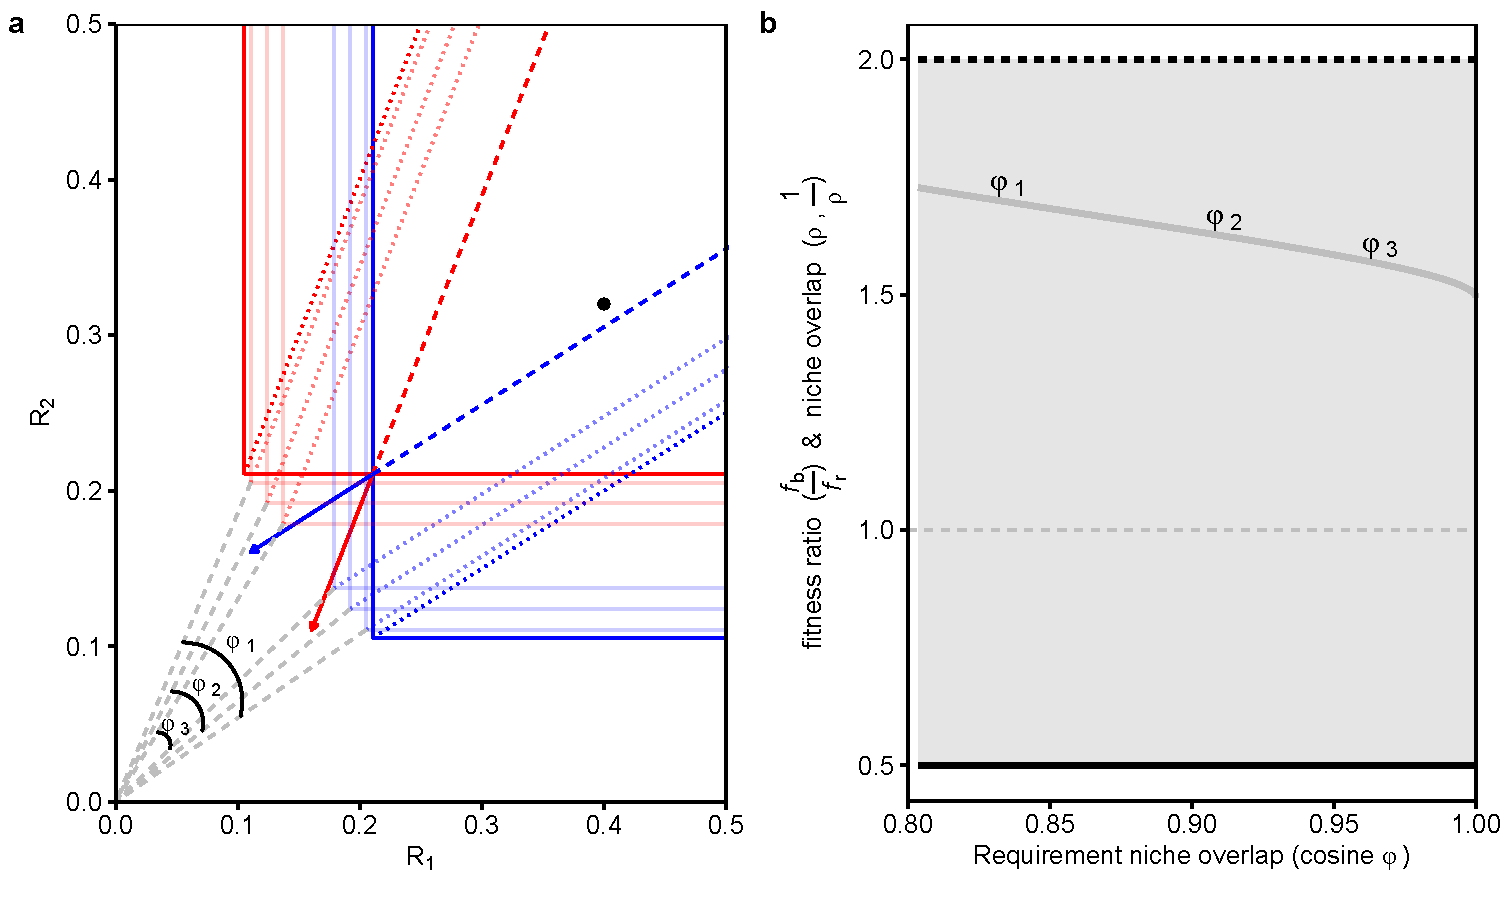
\includegraphics[width=12cm]{Chapter2/require-ms-fig-unfixedequilibrium-appendix.pdf}}
	\caption[The effects of changing requirement niche overlap without fixing the equilibrium resource density for the essential resources model.]
		{\hspace{1mm}The effects of changing requirement niche overlap without fixing the equilibrium resource density for the essential resources model. In (a), the solid red and blue lines are the ZNGIs for each species; the solid lines with arrow heads are the respective impact vectors; and the dashed lines are the inverse of the impact vectors, defining regions of stable coexistence. The additional dotted lines denote the regions in which species switch from being limited by different resources (above blue and below red) to being limited by the same resource (below blue or above red). In (b), the x-axis represents the requirement niche overlap starting from the position given by the solid bold ZNGIs in (a) and ending at complete overlap. The y-axis gives the values of the fitness differences term, $f_{b}/f_{r}$ (solid grey line), and the degree of niche overlap, $\rho$ (solid black line) and $1/\rho$ (dashed black line). The grey shaded area indicates the coexistence region, where $\rho<f_{b}/f_{r}<1/\rho$. For reference, equal fitness, where $f_{b}/f_{r}=1$, is illustrated by the horizontal dashed grey line. The angles given by $\varphi_{1-3}$ in (a) correspond to the respective $\varphi_{1-3}$ in (b).}
	\label{fig:require-appendix-fig-notfix}
\end{figure}

